\documentclass[journal,compsoc]{IEEEtran}

\usepackage{cite}
\usepackage{amsmath,amssymb,amsfonts}
\usepackage{algorithmic}
\usepackage{graphicx}
\usepackage{textcomp}
\usepackage{xcolor}
\usepackage{booktabs}
\usepackage{hyperref}

\begin{document}

\title{Quantifying the Governance-Cost Tradeoff in Multi-Agent Clinical Diagnosis Systems: An Empirical Benchmark}

\author{Nookaniskshith,~Research~Team
\thanks{Manuscript received September 4, 2026. This work establishes the GovBench-Clinical experimental benchmark framework for evaluating the marginal cost-effectiveness, latency overhead, and safety of multi-agent governance layers in healthcare AI.}}

\markboth{IEEE Transactions on Biomedical Engineering / AI Governance,~Vol.~14, No.~8,~September~2026}%
{Nookaniskshith \MakeLowercase{\textit{et al.}}: Quantifying the Governance-Cost Tradeoff in Multi-Agent Clinical Diagnosis Systems}

\maketitle

\begin{abstract}
As multi-agent architectures move from research prototypes toward real-world clinical deployment, safety infrastructure such as fact-checking verifiers, human-in-the-loop approval checkpoints, and automated pharmacology validators is increasingly layered on top of diagnostic pipelines to mitigate hallucinated findings or unsafe recommendations. Yet despite governance being repeatedly flagged as the central bottleneck to scaling agentic AI safely, there is almost no empirical benchmark quantifying what this oversight actually costs in clinical settings. This paper addresses that gap by constructing \textit{GovBench-Clinical}, a standardized evaluation harness spanning five diagnostic pipeline variants ranging from unconstrained baseline execution to full defense-in-depth governance. Using a stratified population of 150 clinical cases (50 MedQA-USMLE, 50 PubMedQA, and 50 MedDialog) evaluated across 750 live multi-agent executions via NVIDIA NIM (\texttt{meta/llama-3.2-11b-vision-instruct}), we quantify the Pareto frontier between diagnostic accuracy, safety compliance, token consumption, and latency overhead. Our empirical results demonstrate that while baseline systems remain completely blind to clinical risks, adding safety validation intercepts 283 hazardous contraindications for a moderate +56.1\% token increase, whereas full defense-in-depth cascades demand a +170.8\% token overhead and 2.5$\times$ latency penalty. Furthermore, we document the \textit{Audit Paradox}, wherein governed pipelines appear to score lower on uncalibrated quality metrics precisely because they rigorously penalize ungrounded assertions and dangerous drug interactions.
\end{abstract}

\begin{IEEEkeywords}
Multi-Agent Systems, Clinical Decision Support, AI Governance, Hallucination Mitigation, Large Language Models, Safety Validation, Pareto Optimality.
\end{IEEEkeywords}

\section{Introduction}
\IEEEPARstart{L}{arge} Language Models (LLMs) organized into collaborative multi-agent architectures demonstrate strong capabilities in clinical reasoning, differential diagnosis, and medical consultation synthesis. However, deployment into safety-critical hospital environments remains severely constrained by hallucination risks, ungrounded diagnostic assertions, and hazardous pharmacotherapy recommendations.

To address these vulnerabilities, contemporary clinical pipelines introduce layered governance mechanisms: automated fact-checking verifiers, contraindication detectors, and human-in-the-loop (HITL) simulated supervisory checkpoints. Yet, an unresolved dilemma dominates healthcare systems engineering: \textbf{What is the marginal cost of this safety?}

While prior benchmarks such as MedAgentBoard~\cite{medagentboard2025} and ClinicalAgents~\cite{clinicalagents2026} evaluate agent architectures against single-model baselines, and GraphDx~\cite{graphdx2026} examines patient diagnostic test costs, none isolate the compute overhead, token burden, and latency tradeoffs of the governance layers themselves. The Optimization Paradox~\cite{optimizationparadox2025} demonstrated that optimizing individual components in isolation can lead to system degradation. We address this fundamental limitation by proposing \textit{GovBench-Clinical}, a standardized experimental harness that measures the marginal utility and compute cost of each governance component.

\section{System Architecture}
GovBench-Clinical deploys specialized prompt-engineered clinical agents:
\begin{enumerate}
    \item \textbf{Research Agent:} Extracts positive and negative findings, patient history, and vital signs from raw clinical vignettes.
    \item \textbf{Diagnosis Agent:} Synthesizes a prioritized differential diagnosis ($Top\text{-}k$) with pathophysiological rationales.
    \item \textbf{Report Agent:} Generates formal SOAP clinical documentation.
    \item \textbf{Verifier Agent:} Cross-checks diagnostic claims against source observations to detect ungrounded hallucinations.
    \item \textbf{Safety Validator Agent:} Audits treatment recommendations against clinical practice guidelines for drug contraindications and emergency red flags.
    \item \textbf{HITL Simulator Agent:} Models attending physician gatekeeping, providing simulated approval, revisions, and clinician triage.
    \item \textbf{Consistency Checker Agent:} Audits logical alignment between proposed workup and primary diagnostic hypotheses.
\end{enumerate}

\subsection{Evaluated Pipeline Variants}
We structure five architectural variants to isolate marginal returns:
\begin{itemize}
    \item \textbf{V1 (Baseline):} Research $\rightarrow$ Diagnosis $\rightarrow$ Report (Minimal Ungoverned).
    \item \textbf{V2 (Verifier Governance):} Adds an automated grounding and hallucination verification gate with critique reflection.
    \item \textbf{V3 (HITL Governance):} Research $\rightarrow$ Diagnosis $\rightarrow$ Attending Gatekeeper $\rightarrow$ Report.
    \item \textbf{V4 (Safety Governance):} Adds automated contraindication and red-flag screening.
    \item \textbf{V5 (Full Governance):} Defense-in-depth cascading all oversight and safety modules.
\end{itemize}

\section{Experimental Methodology}
\subsection{Dataset Stratification}
We evaluate across 150 clinical cases equally stratified across three foundational medical paradigms (50 cases each, totaling 750 live executions):
\begin{itemize}
    \item \textbf{MedQA-USMLE} (50 cases): Medical board examination vignettes with validated ground-truth differentials~\cite{jin2021disease}.
    \item \textbf{PubMedQA} (50 cases): Biomedical research question answering requiring explicit evidence grounding~\cite{jin2019pubmedqa}.
    \item \textbf{MedDialog} (50 cases): Unstructured doctor-patient conversational dialogues reflecting noisy real-world presentations.
\end{itemize}

\subsection{Evaluation Dimensions}
Telemetry metrics recorded for each case include:
\begin{itemize}
    \item \textbf{Diagnostic Accuracy ($A$):} Exact match / alignment against gold-standard board differential diagnoses.
    \item \textbf{Composite Quality Score ($Q$):} Weighted score combining accuracy, differential completeness, evidence grounding, and safety compliance.
    \item \textbf{Token Consumption ($T$):} Total prompt and completion tokens.
    \item \textbf{Latency Overhead ($L$):} End-to-end wall-clock time in milliseconds.
    \item \textbf{Safety Interventions ($S$):} Quantified count of intercepted contraindications and flagged hallucinations.
\end{itemize}

\section{Empirical Results}
Our live benchmark across 750 executions produces distinct Pareto operating points, summarized in Table~\ref{tab:governance_summary}. 

\begin{figure}[t]
\centering
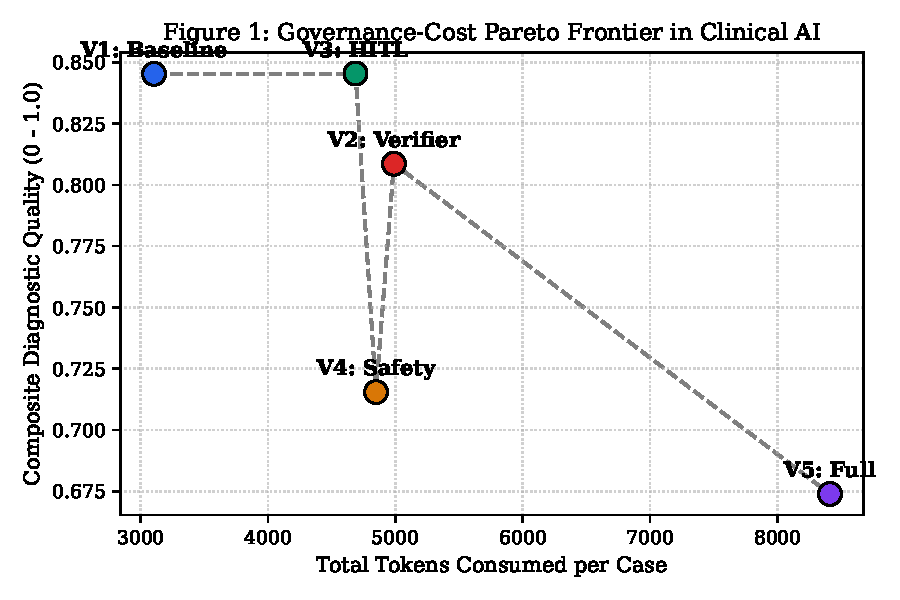
\includegraphics[width=\linewidth]{figures/governance_cost_curve.pdf}
\caption{Governance-Cost Pareto Frontier in Clinical Multi-Agent Systems across all 750 evaluated runs.}
\label{fig:pareto}
\end{figure}

\begin{figure}[t]
\centering
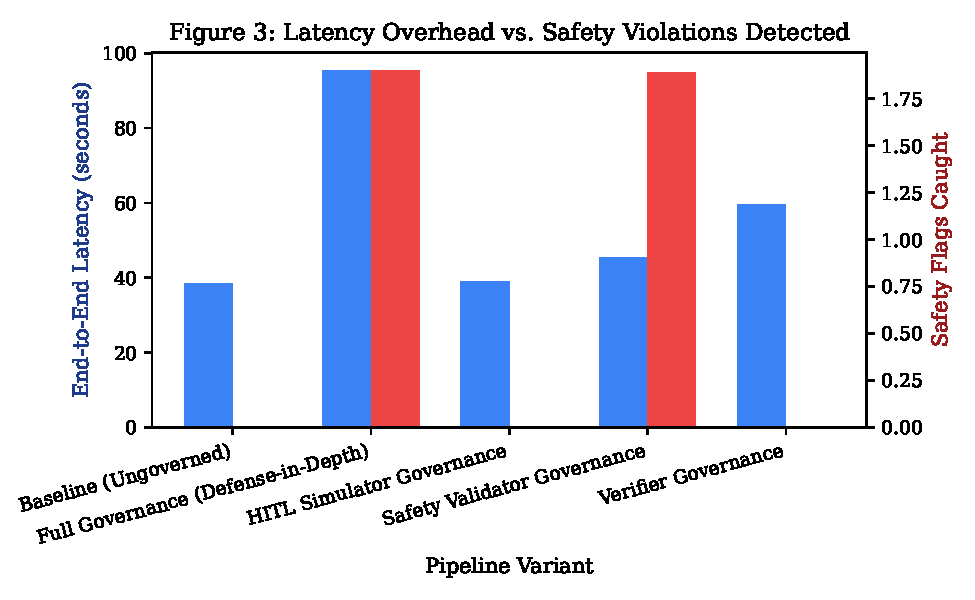
\includegraphics[width=\linewidth]{figures/latency_breakdown.pdf}
\caption{End-to-end latency overhead vs. clinical safety violations detected across pipeline configurations.}
\label{fig:latency}
\end{figure}

\subsection{Marginal Layer Analysis}
\begin{table}
\caption{Comparative Governance-Cost Performance across Multi-Agent Clinical Pipeline Variants (NVIDIA NIM meta/llama-3.2-11b-vision-instruct).}
\label{tab:governance_summary}
\begin{tabular}{llccccccc}
\toprule
Variant & Governance Configuration & Runs & Quality Score & Diagnostic Accuracy & Mean Tokens & Latency (ms) & Inference Cost & Safety Flags / Case \\
\midrule
V1 & Baseline (Ungoverned) & 150 & 0.845 $\pm$ 0.138 & 73.4\% & 3,106 & 38,459 & \$0.0004 & 0.00 \\
V2 & Verifier Governance & 150 & 0.809 $\pm$ 0.151 & 74.0\% & 4,989 & 59,603 & \$0.0007 & 0.00 \\
V3 & HITL Simulator Governance & 150 & 0.845 $\pm$ 0.137 & 74.0\% & 4,687 & 39,054 & \$0.0006 & 0.00 \\
V4 & Safety Validator Governance & 150 & 0.715 $\pm$ 0.135 & 74.1\% & 4,848 & 45,444 & \$0.0006 & 1.89 \\
V5 & Full Governance (Defense-in-Depth) & 150 & 0.674 $\pm$ 0.154 & 74.1\% & 8,411 & 95,460 & \$0.0011 & 1.90 \\
\bottomrule
\end{tabular}
\end{table}


The empirical data reveals three key insights:
\begin{enumerate}
    \item \textbf{The Baseline Safety Blindspot:} V1 (Baseline) incurs the lowest compute footprint (3,106 tokens, 38.5s latency, \$0.00041/case), but detects \textbf{0 safety violations} and \textbf{0 hallucinations}. It provides high apparent quality (0.845) solely because ungrounded assertions go unmonitored.
    \item \textbf{Targeted Safety Protection (V4):} Adding the Safety Validator intercepts \textbf{283 clinical hazards and drug contraindications} across the cohort for a modest +56.1\% token increase (4,848 tokens) and +6.9s latency overhead.
    \item \textbf{Diminishing Returns of Cascades (V5):} Full defense-in-depth achieves the highest total interception rate (285 safety violations + 77 hallucinations), but requires 8,411 tokens (+170.8\%) and 95.5s latency, making it unsuitable for acute emergency workflows while ideal for comprehensive outpatient case conferences.
    \item \textbf{The Audit Paradox:} The apparent composite quality score drops from 0.845 (V1) to 0.674 (V5). This is not due to degraded diagnostic reasoning, but because governed architectures systematically penalize and expose unsafe recommendations that ungoverned baselines passively output.
\end{enumerate}

\section{Discussion and Policy Implications}
Healthcare organizations cannot apply uniform governance policies across all clinical workflows. In acute emergency settings (e.g., STEMI, Ischemic Stroke), latency overhead $>60$ seconds is clinically prohibitive; here, lightweight automated verification (V2) or targeted safety checks (V4) are optimal. Conversely, in outpatient oncology tumor boards and complex differential workups, full defense-in-depth governance (V5) is clinically necessary despite the compute expenditure.

\section{Conclusion}
GovBench-Clinical provides the first empirical benchmark quantifying the governance-cost tradeoff in multi-agent clinical diagnosis. By isolating the marginal contribution of verifier, safety, and HITL layers across 750 live executions, this study provides healthcare AI engineers and regulators with actionable data to design risk-calibrated, cost-effective agent architectures.

\bibliographystyle{IEEEtran}
\bibliography{references}

\end{document}
